% Chapter Template

\chapter{Experimental Results and Conclusion} % Main chapter title

\label{Chapter4} % Change X to a consecutive number; for referencing this chapter elsewhere, use \ref{ChapterX}

\lhead{Chapter 4. \emph{Results}} % Change X to a consecutive number; this is for the header on each page - perhaps a shortened title

%----------------------------------------------------------------------------------------
%	SECTION 1
%----------------------------------------------------------------------------------------

\section{Experimental Evalution}


%-----------------------------------
%	SUBSECTION 1
%-----------------------------------
\subsection{Frequency Response of Hydrophones }

There are a number of wireless communication techniques in underwater channel. These include acoustic, electromagnetic and optical mode. However, these techniques have problems which reduce the efficiency of communication in underwater channel. The reduced efficiency effects data rate, communication range and and Electromagnetic wave does not work well in underwater environment since because of its conduction most of the wave energy is absorbed by the channel.
Similarly optical mode is also not preferred due to scattering of light in underwater channel.
However acoustics is the most popular mode of underwater communication as it is least attenuated by the channel, which allows communication over long ranges. 
\begin{figure}[htbp]
	\centering
		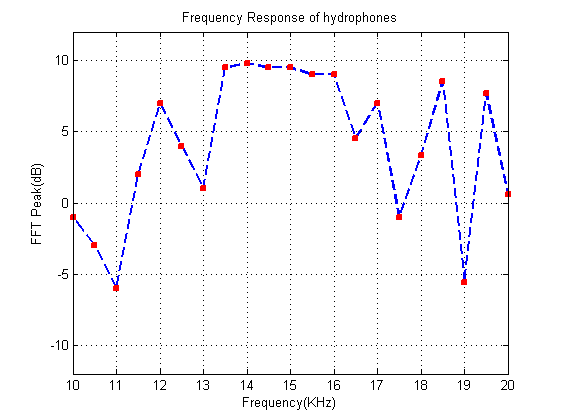
\includegraphics[width=5in]{Figures/Freq_response.png}
		\rule{35em}{0.5pt}
	\caption[Frequency Response of the Hydrophone]{Frequency Response of the Hydrophone.}
	\label{fig:freq}
\end{figure}

%-----------------------------------
%	SUBSECTION 2
%-----------------------------------
\subsection{Directivity Pattern of Hydrophones }

There are a number of wireless communication techniques in underwater channel. These include acoustic, electromagnetic and optical mode. However, these techniques have problems which reduce the efficiency of communication in underwater channel. The reduced efficiency effects data rate, communication range and and Electromagnetic wave does not work well in underwater environment since because of its conduction most of the wave energy is absorbed by the channel.
Similarly optical mode is also not preferred due to scattering of light in underwater channel.
However acoustics is the most popular mode of underwater communication as it is least attenuated by the channel, which allows communication over long ranges. 

%-----------------------------------
%	SUBSECTION 3
%-----------------------------------
\subsection{Transmission Range of Hydrophones }

There are a number of wireless communication techniques in underwater channel. These include acoustic, electromagnetic and optical mode. However, these techniques have problems which reduce the efficiency of communication in underwater channel. The reduced efficiency effects data rate, communication range and and Electromagnetic wave does not work well in underwater environment since because of its conduction most of the wave energy is absorbed by the channel.
Similarly optical mode is also not preferred due to scattering of light in underwater channel.
However acoustics is the most popular mode of underwater communication as it is least attenuated by the channel, which allows communication over long ranges. 
\begin{figure}[htbp]
	\centering
		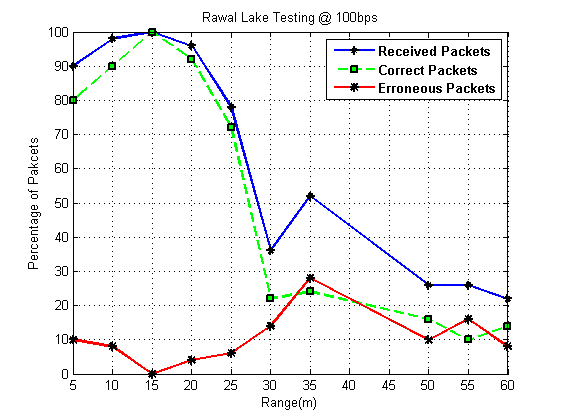
\includegraphics[width=5in]{Figures/Rawal_dam.png}
		\rule{35em}{0.5pt}
	\caption[Range Testing of the Hydrophones]{Range Testing of the Hydrophones.}
	\label{fig:rawal}
\end{figure}

%-----------------------------------
%	SUBSECTION 4
%-----------------------------------
\subsection{Evaluation of Testbed }

In this section we would evaluate the overall performance of our platform in terms of automation and communications so as to validate the claims made in previous sections.
1-	Evaluation Setup: the Platform evaluations setup is as show in the figure. We perform the experiments in specially designed pool measuring 20’ X 10’ in length and width respectively. For each physical point we send 500 packets and then evaluate the performance in terms of packet sent, received and lost. 
2-	Figure O shows the user interfaces(UI) for our web front. Figure Oa show the home page and Ob shows the experimentation page. You are required to fill in the details 

\begin{figure}[htbp]
	\centering
		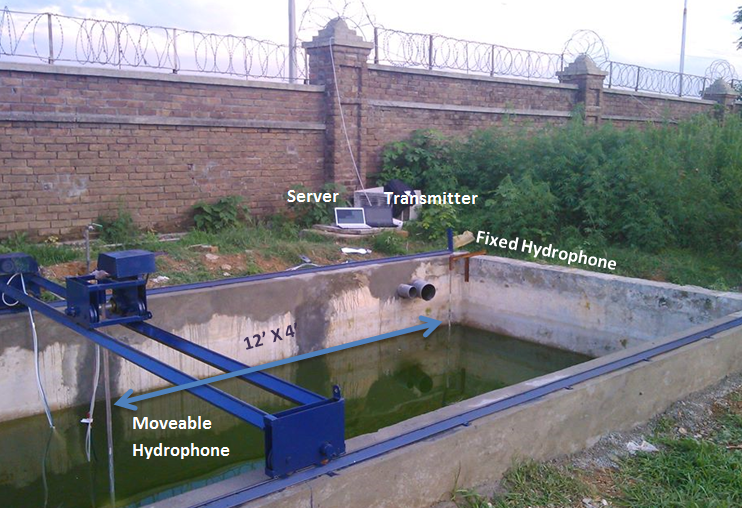
\includegraphics[width=5in]{Figures/setup11.png}
		\rule{35em}{0.5pt}
	\caption[Evaluation Setup of the Testbed]{Evaluation Setup of the Testbed.}
	\label{fig:evaluation}
\end{figure}


\begin{figure}[htbp]
	\centering
		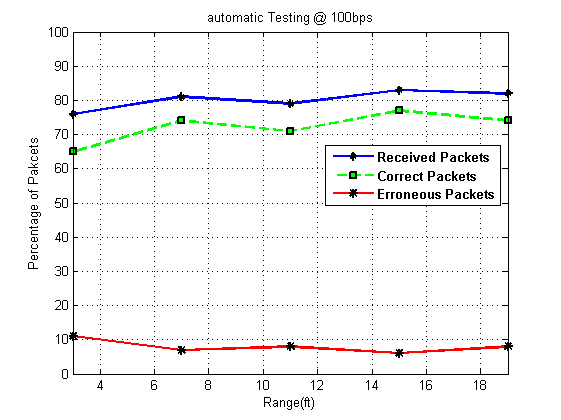
\includegraphics[width=5in]{Figures/results.png}
		\rule{35em}{0.5pt}
	\caption[Evaluation Result of the Testbed]{Evaluation Result of the Testbed.}
	\label{fig:evaluation_results}
\end{figure}


%----------------------------------------------------------------------------------------
%	SECTION 2
%----------------------------------------------------------------------------------------

\section{Conclusion and Future Work}


%-----------------------------------
%	SUBSECTION 1
%-----------------------------------
\subsection{Conclusion }

There are a number of wireless communication techniques in underwater channel. These include acoustic, electromagnetic and optical mode. However, these techniques have problems which reduce the efficiency of communication in underwater channel. The reduced efficiency effects data rate, communication range and and Electromagnetic wave does not work well in underwater environment since because of its conduction most of the wave energy is absorbed by the channel.
Similarly optical mode is also not preferred due to scattering of light in underwater channel.
However acoustics is the most popular mode of underwater communication as it is least attenuated by the channel, which allows communication over long ranges. 

%-----------------------------------
%	SUBSECTION 2
%-----------------------------------
\subsection{Future Work }

There are a number of wireless communication techniques in underwater channel. These include acoustic, electromagnetic and optical mode. However, these techniques have problems which reduce the efficiency of communication in underwater channel. The reduced efficiency effects data rate, communication range and and Electromagnetic wave does not work well in underwater environment since because of its conduction most of the wave energy is absorbed by the channel.
Similarly optical mode is also not preferred due to scattering of light in underwater channel.
However acoustics is the most popular mode of underwater communication as it is least attenuated by the channel, which allows communication over long ranges. 

